%% Source Template:
%% Copyright (C) 2014 by Pascal Richter, Elena Botoeva, Richard Barnard, and Dirk Surmann
%% 
%% This file may be distributed and/or modified under the
%% conditions of the LaTeX Project Public License, either
%% version 2.0 of this license or (at your option) any later
%% version. The latest version of this license is in:
%% 
%% http://www.latex-project.org/lppl.txt
%% 
%% and version 2.0 or later is part of all distributions of
%% LaTeX version 2013/12/01 or later.
%% 

\documentclass[20pt, a1paper, portrait, margin=0mm, innermargin=10mm,
    titleinnersep=0mm, blocktitleinnersep=0mm,
    blocktitlewidthratio=08, blocktitlemaxwidth=35cm ,blockbodyinnersep=8mm,
    blockverticalspace=10mm,colspace=5mm, subcolspace=0mm,noteinnersep=3mm]
{tikzposter}

% Choose Layout
\usetheme{Autumn}

% Additonal packages
\usepackage{wrapfig}
\usepackage{floatflt}
\usepackage{multicol}
\usepackage{placeins}
\usepackage[T1]{fontenc}

% Set block style
\useblockstyle[titlewidthscale=1, bodywidthscale=1, titlecenter,
    titleoffsetx=0pt, titleoffsety=0pt, bodyoffsetx=0pt, bodyoffsety=30pt,
    bodyverticalshift=0pt, roundedcorners=5, linewidth=0.4cm,
    titleinnersep=10mm, bodyinnersep=10mm]{Default}

\usetitlestyle[titletoblockverticalspace=10mm]{Filled}

\tikzposterlatexaffectionproofoff


% Header
\title{\textcolor{colorThree}{\fontsize{2.3cm}{1em}\selectfont 
       Gravitational Waves from Neutron Stars}}

\author{Gregory Ashton, supervised by D.I. Jones \& R. Prix \\
    {\Large G.Ashton@soton.ac.uk}}

\institute{University of Southampton }

\begin{document}

 % Title block with title, author, logo, etc.
\maketitle


 %\block{Introduction}{
%}
\begin{columns}
 % FIRST column
\newcommand{\mycolwidth}{0.5}
\column{\mycolwidth}
\block[]{I: What is a \emph{gravitational wave}?}{

In 1916 Einstein formulated his theory of gravity, general relativity. Like all
good theories it made several important predictions. All but one of these
predictions have been tested and agree with the theory exceptionally well. The
final prediction left to test is the existence of \emph{gravitational waves}.


General relativity unified the ideas of space and time into a single object
which we call \emph{spacetime}. Spacetime is a dynamic object that can interact
with matter. We can picture this by imagining a stretched rubber sheet on which
we place heavy weights, this creates wells in the sheet. In this picture the rubber
sheet is spacetime while the weights are large masses e.g. stars, black holes. The two react
to each dynamically, this can be summarised as:
\vspace{2mm}
\begin{quotation}
    {
\emph{\textbf{``Spacetime tells matter how to move; matter
tells spacetime how to curve."} - J. Wheeler}}
\end{quotation}
\vspace{2mm}

\begin{wrapfigure}[6]{l}{0.43\linewidth}
    \vspace{-10mm}
\begin{tikzfigure}
\centering

\includegraphics[width=\linewidth]{img/star_with_GW-crop}
\end{tikzfigure}
\end{wrapfigure}
When a large mass which is not symmetric rotates it causes the spacetime to
ripple as illustrated in the figure on the left. These ripples
are gravitational waves, there is very strong evidence that they exist, but they
have not yet been directly observed.

}



 % SECOND column
\column{\mycolwidth}

\block{II: What is a \emph{neutron star}?}{

\begin{wrapfigure}[9]{r}{0.38\linewidth}
    \vspace{-10mm}
\begin{tikzfigure}
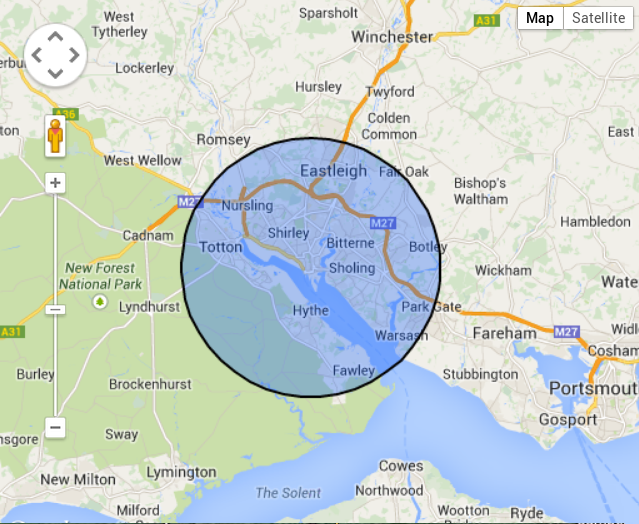
\includegraphics[width=\linewidth]{img/southampton}
\label{fig: map}
\end{tikzfigure}
\end{wrapfigure}


Stars like our sun are in an equilibrium between the outward force from burning
nuclear fuel in their core and collapse due to their own gravity.  When they
run out of fuel they collapse, some of them collapse to form a neutron star.
They have a mass about that of our sun, but have a radius of about 10km, this
makes them extremely dense. This is like compressing the sun into a sphere
roughly the size of Southampton.
\vspace{4mm}
\begin{wrapfigure}[11]{l}{0.5\linewidth}
    \vspace{-15mm}
\begin{tikzfigure}
\centering
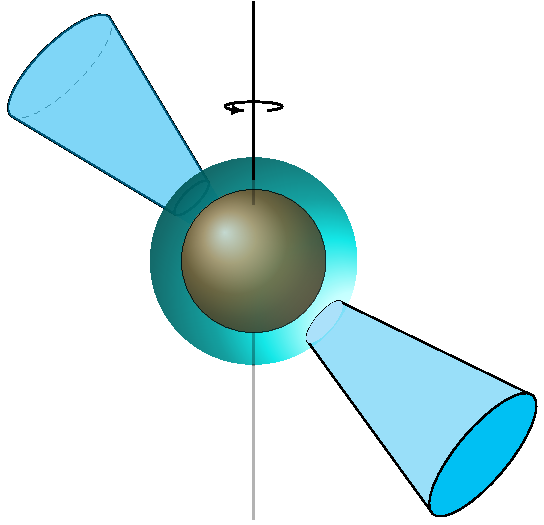
\includegraphics[width=\linewidth]{img/star-crop}
\end{tikzfigure}
\end{wrapfigure}

We see some neutron stars as pulses of electromagnetic light. This is caused by
radiation streaming out in thin beams which flash over the earth like the beams
from a lighthouse, illustrated on the left.  Neutron stars contain lots of
interesting physics such as superfluids and massive magnetic fields. Crucially,
if they are misshapen then they may emit gravitational waves. 
\vspace{2.3mm}
}

\end{columns}

\block[]{III: Searching for gravitational waves}{

\begin{minipage}[t]{0.49\linewidth}

A gravitational wave will periodically stretch and squeeze space in the two
directions perpendicular to its direction of travel. In the figure below we 
show this effect on a circle. 
{
\begin{tikzfigure}
    \vspace{-10mm}
    \centering
    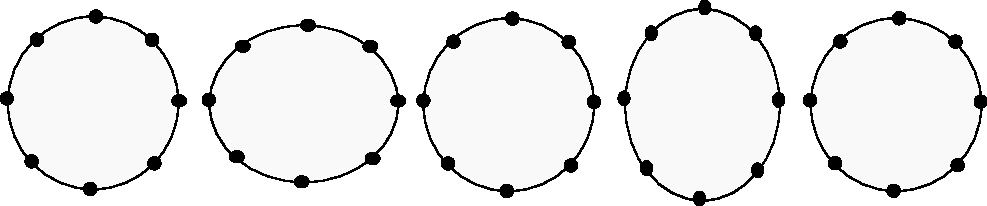
\includegraphics[width=0.5\linewidth]{img/RingOfParticles}
\end{tikzfigure}
}

\begin{wrapfigure}{r}{0.5\linewidth}
    \vspace{-10mm}
\begin{tikzfigure}
\centering
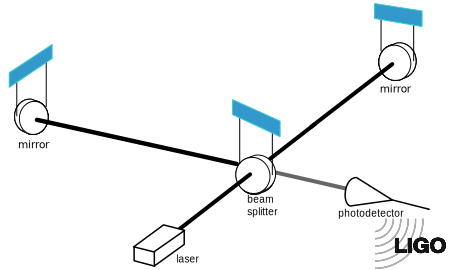
\includegraphics[width=\linewidth]{img/Ligo}
\end{tikzfigure}
\end{wrapfigure}

To detect gravitational waves we can use a laser interferometer. These split a
laser beam and send it off in two different directions; both beams are then
bounced off a mirror and return to the start. Both beams should have travelled
the same distance and so should return at the same time. However, if a
gravitational wave passed through during the experiment, they will not both
return at the same time. 

\end{minipage}
\hspace{2mm}
\vrule{}
\hspace{2mm}
\begin{minipage}[t]{0.49\linewidth}

The problem is that the difference between the two beams is tiny.  To put
it in perspective, it's like trying to measure if a human being has grown by a
single atom. We have built enormous interferometers in the hope of measuring
gravitational waves, for example here is one of the 4 km long LIGO detectors:
\begin{tikzfigure}
   \vspace{-3mm}
\centering
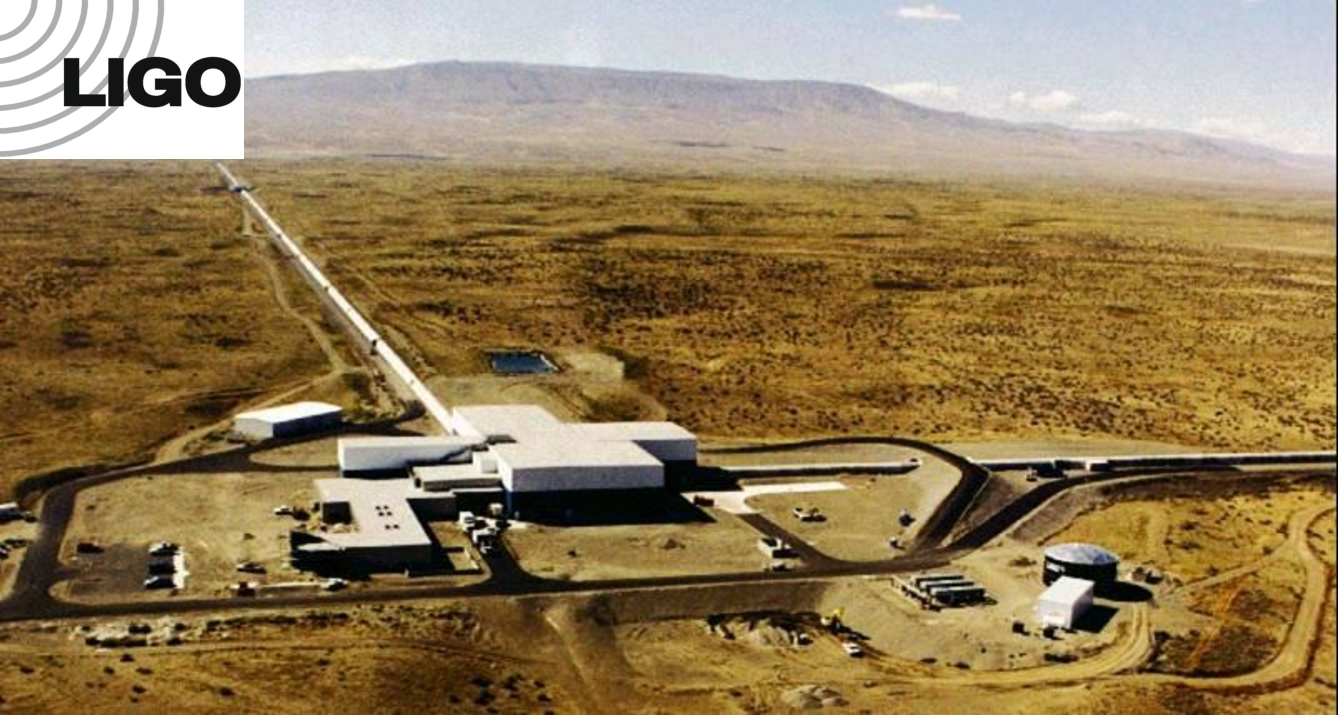
\includegraphics[width=0.8\linewidth]{img/Hanford1_with_logo}
\end{tikzfigure}
You can find out more about this project at: \textcolor{blue}{www.bit.do/LIGO}


\end{minipage}
}

\block[]{IV: Searching for signals from neutron stars}{

\begin{wrapfigure}{r}{0.355\linewidth}
    \vspace{-33mm}
\begin{tikzfigure}
\centering
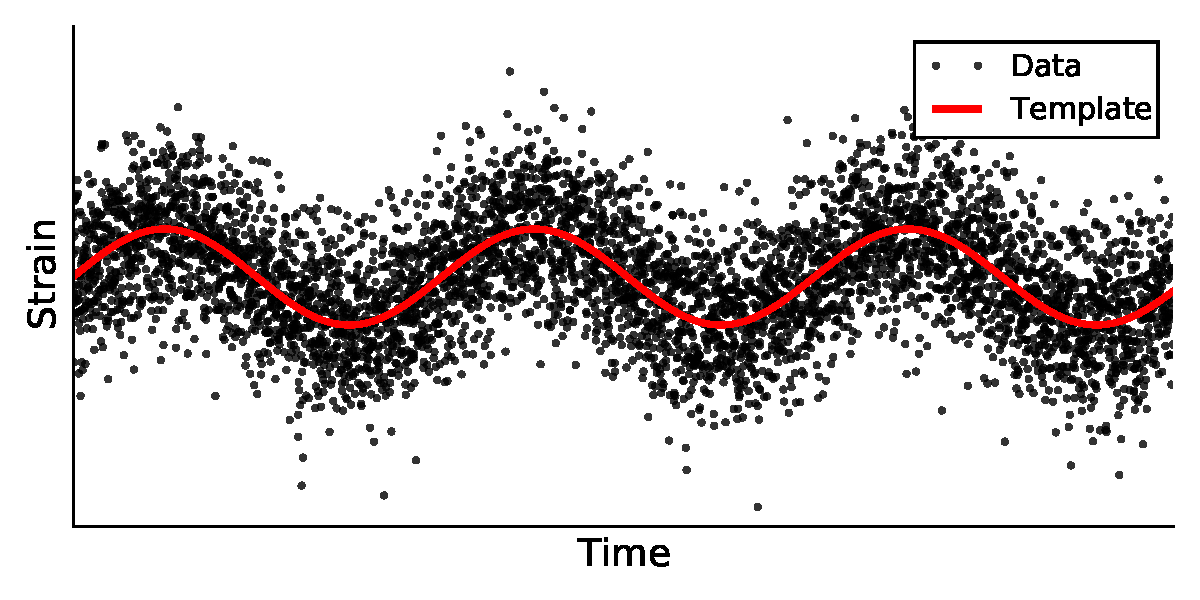
\includegraphics[width=\linewidth]{img/CGW_example}
\end{tikzfigure}
\end{wrapfigure}

The signals we are searching for will be hidden in the  detector noise from
seismic activity and other sources. To search for it, we have to make an
educated guess for what the signal will look like, this is called a template.
The template is then compared to the data like in the graph on the right. This
process relies on the ability of the template to match the signal in the data.
Using the correct template is crucial to finding the signal. Unfortunately it
is possible that real gravitational wave signals will contain noise from the
neutron star itself.  This noise can look just like the detector noise. I am
trying to test how bad this effect will be and develop methods to improve our
chances of detection.

}

\begin{columns}

\column{0.5}
\block[]{V: Gravitational waves astronomy}{

Aside from testing Einstein's general relativity, gravitational waves will
allow us to explore the universe in a new way. Traditional astronomy observes
electromagnetic radiation from distant objects. This means we can only observe
the outside of hot, light emitting objects. With gravitational wave astronomy
we may be able to observe more of the difficult to explore areas of physics
such as black holes, neutron stars, and maybe even the big bang. 

}

\column{0.5}
\block[]{VI: Conclusions}{

Scientists from around the world are trying to detect gravitational waves.
Finding these is crucial evidence for Einstein's theory of gravity, general
relativity. Here in the gravity group of Southampton, we are helping by
modelling neutron stars. We use these models to predict what the signals may
look like. I am interested in finding out what happens when the signals include
noise from the neutron star.


\vspace{4.0mm}
}
\end{columns}

\end{document}



\endinput
%%
